\documentclass[
a4paper, % Paper size, use either a4paper or letterpaper
12pt, % Default font size, the template is designed to look good at 12pt so it's best not to change this
%unnumberedsections, % Uncomment for no section numbering
]{article}
\usepackage[a4paper,top=0.4cm, bottom=0.8cm, left=1.6cm, right=1.6cm]{geometry}

\usepackage{cmap} % make PDF files searchable and copy-able
\usepackage[utf8]{inputenc}
\usepackage[english,russian]{babel}

\usepackage{amssymb,amsmath}
\renewcommand {\phi}{\varphi}
\usepackage{mathtext}

\usepackage{libertine}
\usepackage[libertine]{newtxmath}

\usepackage{graphicx} % Required for inserting images
\graphicspath{{./img/}} % Destination of images

\usepackage{subcaption}
\usepackage{wrapfig}

\usepackage{hyperref}

\usepackage{xcolor}



% opening
\title{
	\textcolor{cyan}{Отчет о выполнении лабораторной работы 3.2.5}
	\\
	Свободные и вынужденные колебания в электрическом контуре
}
\author{Шубин Владислав, Байбулатов Амир}
%\date{Ноябрь 2023}

\begin{document}    
	
	\maketitle
	
	\section{Аннотация}
	
	В работе исследуется параллельный колебательный контур: определяется зависимость периода свободных колебаний контура от емкости; определяется зависимость логарифмического декремента затухания от сопротивления; исследуется построение резонансных кривых колебательного контура: АЧХ и ФЧХ.
	
	\section{Теоретические сведения}
	
	\begin{figure}[h]
		\centering
		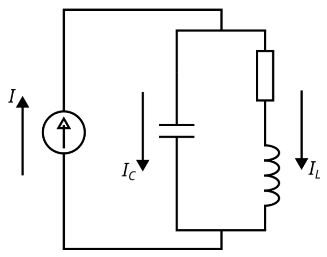
\includegraphics[width=0.74\linewidth]{img/scheme}
		\caption[RLC]{Схема RLC контура}
		\label{fig:scheme}
	\end{figure}
	
	%\begin{wrapfigure}{r}{0.5\textwidth}
	%	\begin{center}
	%		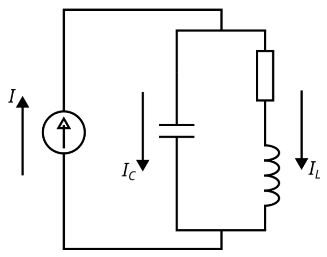
\includegraphics[width=0.4\linewidth]{img/scheme}
	%	\end{center}
	%	\caption[RLC]{Схема RLC контура}
	%	\label{fig:scheme}
	%\end{wrapfigure}
	
	\noindent Для RLC контура \ref{fig:scheme} применим 2 правило Кирхгофа:
	\begin{equation}
		RI + U_C + L\frac{dI}{dt} = 0.
	\end{equation}
	Подставив в уравнение (1) выражение для тока через 1-ое правило Кирхгофа, и разделив обе части уравнения на $CL$, получим:
	\begin{equation}
		\frac{d^2U_C}{dt^2} + \frac{R}{L} \frac{dU_C}{dt} + \frac{U_C}{CL}.
	\end{equation}
	Произведём замены $\gamma = \frac{R}{2L}$ -- коэффициент затухания, $\omega_0^2 = \frac{1}{LC}$ -- собственная круговая частота, $T_0 = \frac{2\pi}{\omega_0} = 2\pi \sqrt{LC}$ -- период собственных колебаний. Тогда уравнение (2) примет вид:
	\begin{equation}
		\ddot{U_C} + 2 \gamma \dot{U_C} + \omega_0^2U_C = 0,
	\end{equation}
	где точкой обозначено дифференцирование по времени. Будем искать решение данного дифференциального уравнения в классе функций следующего вида:
	$$U_C(t) = U(t)e^{- \gamma t}.$$
	Получим:
	\begin{equation}
		\ddot{U} + \omega_1^2 U = 0, \text{	где	} \omega_1^2 = \omega_0^2-\gamma^2
	\end{equation}
	Для случая $\gamma < \omega_0$ в силу того, что $\omega_1 > 0$, получим:
	\begin{equation}
		U_C(t) = U_0 \cdot e^{-\gamma t} \cos{(\omega_1 t + \varphi_0)}.
	\end{equation}
	Для получения фазовой траектории представим формулу (6) в другом виде:
	\begin{equation}
		U_C(t) = e^{-\gamma t}(a \cos{\omega_1 t} + b\sin{\omega_1 t}),
	\end{equation}
	где $a$ и $b$ получаются по формулам:
	$$a = U_0 \text{cos} \varphi_0, \qquad b = - U_0 \text{sin} \varphi_0.$$
	В более удобном виде запишем выражения для напряжения на конденсаторе и токе через катушку:
	\begin{equation}
		U_C (t) = U_{C0} \cdot e^{-\gamma t} (\cos{\omega_1 t + \frac{\gamma}{\omega_1}} \sin{\omega_1 t}),
	\end{equation}
	\begin{equation}
		I(t) = C\dot{U_C}= - \frac{U_{C0}}{\rho} \frac{\omega_0}{\omega_1} e^{-\gamma t} \sin{\omega_1 t}.
	\end{equation}
	Введём некоторые характеристики колебательного движения:
	\begin{equation}
		\tau = \frac{1}{\gamma} = \frac{2L}{R},
	\end{equation}
	где $\tau$ -- время затухания (время, за которое амплитуда колебаний уменьшается в $e$ раз).
	\begin{equation}
		\Theta = \text{ln} \frac{U_k}{U_{k+1}} = \gamma T_1 = \frac{1}{N_\tau} = \frac{1}{n} \text{ln} \frac{U_k}{U_{k+n}}, 
	\end{equation}
	где $\Theta$ -- логарифмический декремент затухания, $U_k$ и $U_{k+1}$ -- два последовательных максимальных отклонения величины в одну сторону, $N_\tau$ -- число полных колебаний за время затухания $\tau$.
	
	Теперь рассмотрим случай \textit{вынужденных колебаний} под действием внешней внешнего синусоидального источника. Для этого воспользуемся методом \textit{комплексных амплитуд} для схемы на рис.\ref{fig:scheme}:
	\begin{equation}
		\ddot{I} + 2 \gamma \dot{I} + \omega^2 I = - \varepsilon \frac{\Omega}{L} e^{i\Omega t}.
	\end{equation}
	Решая данное дифференциальное уравнение получим решение:
	\begin{equation}
		I = B\cdot e^{-\gamma t} \sin{(\omega t - \Theta)} + \frac{\varepsilon_0 \Omega}{L \phi_0} \sin{(\Omega t - \varphi)}.
	\end{equation}
	Нетрудно видеть, что частота резонанса будет определяться формулой:
	\begin{equation}
		\omega_0 = \frac{1}{2 \pi \sqrt{LC}}.
	\end{equation}
	
	
	\newpage
	
	\section{Оборудование и инструментальные погрешности}
	
	\textbf{Оборудование}: осциллограф АКТАКОМ ADS-6142H, генератор сигналов специальной формы АКИП-3409/4, магазин сопротивления МСР-60, магазин емкости Р5025, магазин индуктивности Р567 типа
	МИСП, соединительная коробка с шунтирующей емкостью, соединительные одножильные и коаксиальные провода.
	
	\section{Результаты измерений и обработка данных}
	
	\subsection{Описание экспериментальной установки}
	Схема установки для исследования колебаний приведена на рис.\ref{fig:electricalcircuit}.
	Колебательный контур состоит из постоянной индуктивности $L$ с активным сопротивлением $R_L$, переменной емкости $C$ и сопротивления $R$. Картина колебаний напряжения на емкости наблюдается на экране двухканального осциллографа. Для возбуждения затухающих колебаний используется генератор сигналов специальной
	формы. Сигнал с генератора поступает через конденсатор $C_1$ на вход колебательного контура. Данная емкость необходима чтобы выходной импеданс генератора был много меньше импеданса колебательного контура и не влиял на процессы, проходящие в контуре.
	
	\begin{figure}[h]
		\centering
		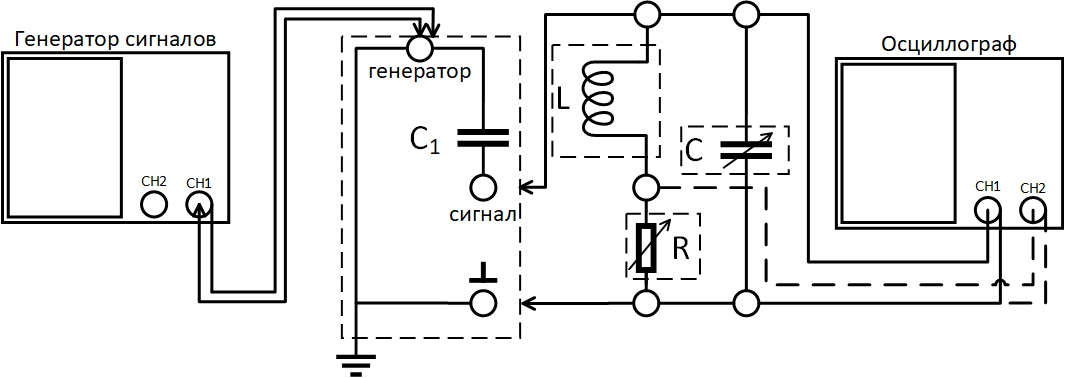
\includegraphics[scale=0.4]{img/electrical_circuit}
		\caption{Схема установки для исследования вынужденных колебаний}
		\label{fig:electricalcircuit}
	\end{figure}
	
	\noindent
	Установка предназначена для исследования не только возбужденных, но и свободных колебаний в электрической цепи.
	
	\begin{figure}[h]
		\centering
		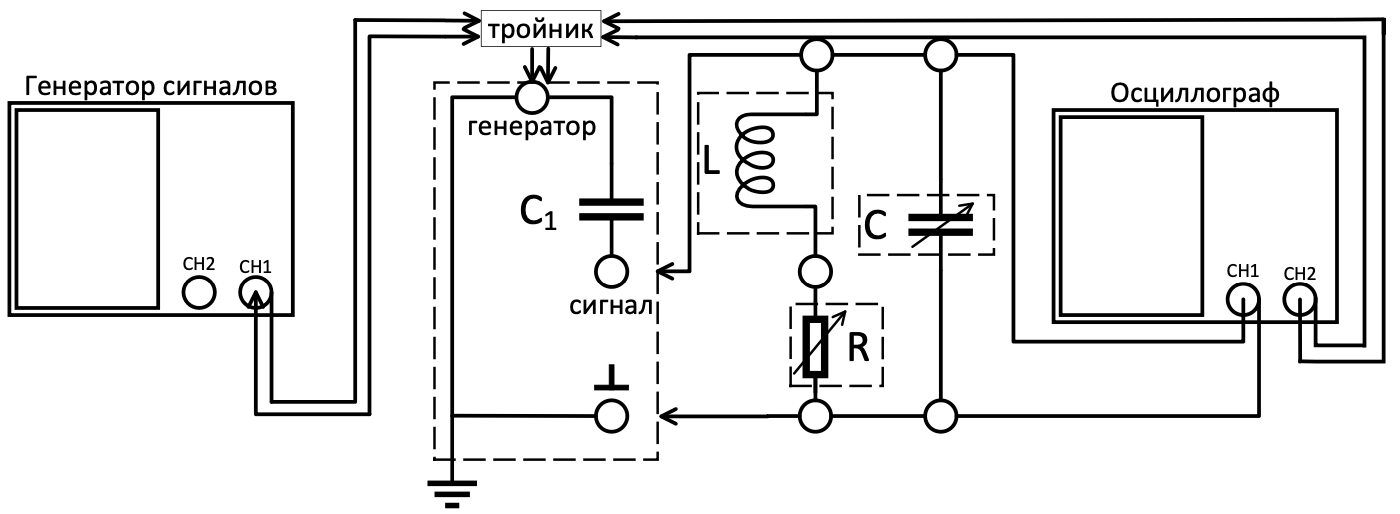
\includegraphics[width=0.90\linewidth]{img/PhaseAmplCharCircuit}
		\caption{Схема установки для исследования АЧХ и ФЧХ}
		\label{fig:phaseamplcharcircuit}
	\end{figure}
	
	\newpage
	
	\subsection{Характеристики системы}
	
	L = 100 мГн\\
	R = 0.001 Ом
	
	\subsection{Предварительные расчеты:}
	\begin{equation}
		C_0 = 7.6 * 10^{-10} \text{Ф}
	\end{equation}
	\begin{equation}
		R_{\text{cr}} = 8165 \:\text{Ом}
	\end{equation}
	\subsection{Практическая часть}
	
	

	\begin{table}[h]
		\centering
		\begin{tabular}{|c|c|c|c|}
			\hline
			№ & С, мкф & $T_\text{теор}$, мкс & $T_\text{практ}$, мкс \\
			\hline
			1 & 0.002 & 88.8 & 88.2 \\
			\hline
			2 & 0.003 & 108.8 & 100.1 \\
			\hline
			3 & 0.004 & 125.6 & 115.1 \\
			\hline
			4 & 0.005 & 140.4 & 130.3 \\
			\hline
			5 & 0.006 & 153.8 & 140.1 \\
			\hline
		\end{tabular}
		\caption{Результаты измерений}
	\end{table}
	
	\begin{figure}[h]
		\centering
		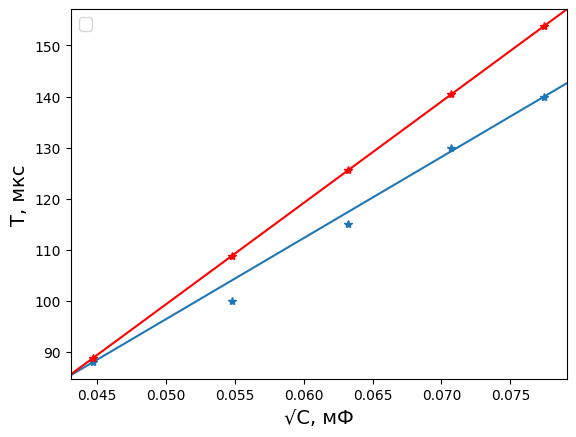
\includegraphics[width=0.68\linewidth]{img/TsqrtC}
		\caption{График зависимости периода собственных колебаний от корня из ёмкости системы}
		\label{fig:tsqrtc}
	\end{figure}
	
	\begin{table}[h]
		\centering
		\begin{tabular}{|c|c|c|c|c|}
			\hline
			№ & R, Ом & $U_1$, мВ & $U_2$, мВ & $\theta$ \\
			\hline
			1 & 408.2 & 176.0 & 260 & 0.39 \\
			\hline
			2 & 458.2 & 216.0 & 332.0 & 0.43 \\
			\hline
			3 & 688.2 & 112.0 & 204.0 & 0.6 \\
			\hline
			4 & 988.2 & 106.0 & 248.0 & 0.85\\
			\hline
			5 & 1488.2 & 124.0 & 423.0 & 1.23\\
			\hline
			5 & 1888.2 & 75.0 & 338.0 & 1.51\\
			\hline
		\end{tabular}
		\caption{Результаты измерений декрементов}
	\end{table}
	
	\newpage
	
	\section{Заключение}
	\begin{enumerate}
		\item В ходе сравнения зависимости с теоретической была обнаружена некоторая небольшая ёмкость колебательной системы (исключая магазин ёмкостей), которая смещает зависимость $T(C)$ на некоторую константу, однако, достаточно мала, чтобы изменить характер зависимости (изменений установить не удалось).
		
		\item Удалось снять зависимость логарифмического декремента затухания от активного сопротивления цепи (погрешность составила порядка $5\%$), основной причиной такой погрешности послужили наводки, которые <<размазывали сигнал>>, особенно на пиках амплитуд, делая невозможным поддерживать точность на уровне точности приборов. График данной зависимости в линеализирующих координатах:
		
		\item Определили критическое сопротивление, при котором характер колебаний меняется на апериодический, тремя способами: теоретическим $R_\text{кр} = 8,16 \pm 0,12 \ \text{кОм},$ по наклону графика зависимости логарифмического декремента затухания от сопротивления цепи $R_\text{кр} = 6,2 \pm 0,4 \ \text{кОм},$ с помощью наблюдением за картиной колебаний $R_\text{кр} = 3 \ \text{кОм}.$ Как видим, значения довольно сильно отличаются, это связано с неточностью $R_\text{кр}$ по своей природе.
		
		\item Были сняты АЧХ и ФЧХ для вынужденных колебаний в цепи, проведена аппроксимация соответствующих теоретических зависимостей к экспериментальным точкам, функции из теории хорошо ложатся на точки, однако при этих измерениях возникли ещё большие наводки, сделали случайную погрешность кратно больше системной ($\sigma_\text{случ} \sim 7 \sigma_\text{сист}$), однако из-за аппроксимации они не имею большого вклада в итоговые результаты.
		
		\item Удалось определить логарифмические декременты затухания по установлению и затуханию вынужденных колебаний, получены значения декремента для двух значений сопротивления магазина:
		
		при $R = 140 \ \text{Ом}$ $\Theta_\text{затух} = 0.19 \pm 0.015;$ $\Theta_\text{устан} = 0.179 \pm 0.01$, 
		
		при $R = 280 \ \text{Ом}$ $\Theta_\text{затух} = 0.293 \pm 0.013;$ $\Theta_\text{устан} = 0.29 \pm 0.03$. 
		
		Как видим, значения хорошо совпадают в пределах погрешностей. 
		
	\end{enumerate}
	
	
\end{document}
